%-----------------------------------------------------------------------
% APPENDIX: Member Certificates and Resumes
%-----------------------------------------------------------------------
\chapter{Member Certificates and Resumes}
\label{chap:member-certs}

%
% \certentry{Issuer}{Year}{Description text}{image-path}
% Places description and certificate image together on the same page.
%
\newcommand{\certentry}[4]{%
  \noindent\begin{minipage}{\linewidth}
    \small\textbf{Issuing Body:}~#1 \quad \textbf{Completion:}~#2\par
    \smallskip
    \small #3\par
    \vspace{0.6em}
    \centering
    \includegraphics[width=0.90\linewidth,height=0.60\textheight,keepaspectratio]{#4}%
  \end{minipage}%
  \par\bigskip
}

%
% \resumeentry{image-path}
% Full-page resume image.
%
\newcommand{\resumeentry}[1]{%
  \noindent\begin{minipage}{\linewidth}
    \centering
    \includegraphics[width=\linewidth,height=0.92\textheight,keepaspectratio]{#1}%
  \end{minipage}%
  \par
}

\noindent
This appendix presents the professional certifications and academic achievements
of each project member, followed by their individual curriculum vitae.
All certificates listed below were earned during the B.Tech.\ programme and are
directly relevant to the technical domains addressed in this project.


\vspace{0.8em}
\noindent{\large\textbf{Certificate Index}}
\vspace{0.4em}

\renewcommand{\arraystretch}{1.2}
\begin{longtable}{@{} l @{\hspace{1.2em}} l @{\hspace{2em}} l @{}}
  \toprule
  \textbf{Ref.} & \textbf{Certificate / Document} & \textbf{Member} \\
  \midrule
  \endfirsthead
  \toprule
  \textbf{Ref.} & \textbf{Certificate / Document} & \textbf{Member} \\
  \midrule
  \endhead
  \midrule\multicolumn{3}{r}{\small\itshape Continued\ldots}\\
  \endfoot
  \bottomrule
  \endlastfoot
  %--- A ---
  \multicolumn{3}{@{}l@{}}{\rule{0pt}{2.2ex}\textbf{A \textemdash{} Shubh Rajesh Shah}} \\[2pt]
  A.1  & AI--ML Virtual Internship (Agartas)         & Shubh R.\ Shah \\
  A.2  & Cisco / AICTE AI--ML Internship             & Shubh R.\ Shah \\
  A.3  & Virtual Internship Certificate              & Shubh R.\ Shah \\
  A.4  & Python Programming                          & Shubh R.\ Shah \\
  A.5  & C Programming                               & Shubh R.\ Shah \\
  A.6  & Java Programming                            & Shubh R.\ Shah \\
  A.7  & PSQL Spoken Tutorial                        & Shubh R.\ Shah \\
  A.8  & Internship Appointment Letter               & Shubh R.\ Shah \\
  A.9  & Additional Participant Certificate          & Shubh R.\ Shah \\
  A.10 & IJARCCE Research Publication Certificate   & Shubh R.\ Shah \\
  A.11 & Curriculum Vitae (Resume)                  & Shubh R.\ Shah \\[6pt]
  %--- B ---
  \multicolumn{3}{@{}l@{}}{\rule{0pt}{2.2ex}\textbf{B \textemdash{} Anurag Mrityunjay Kumar}} \\[2pt]
  B.1  & AI--ML Certification                        & Anurag M.\ Kumar \\
  B.2  & Internship Appointment Letter               & Anurag M.\ Kumar \\
  B.3  & C Programming                               & Anurag M.\ Kumar \\
  B.4  & R Training Certificate                      & Anurag M.\ Kumar \\
  B.5  & CCNA -- Introduction to Networking          & Anurag M.\ Kumar \\
  B.6  & Deloitte Data Analytics Certification       & Anurag M.\ Kumar \\
  B.7  & DSA Certificate                             & Anurag M.\ Kumar \\
  B.8  & Infosys CSR -- Data Analytics (ICT Academy) & Anurag M.\ Kumar \\
  B.9  & Java Programming                            & Anurag M.\ Kumar \\
  B.10 & JavaScript Programming                      & Anurag M.\ Kumar \\
  B.11 & Python Programming                          & Anurag M.\ Kumar \\
  B.12 & IJARCCE Research Publication Certificate   & Anurag M.\ Kumar \\
  B.13 & Curriculum Vitae (Resume)                  & Anurag M.\ Kumar \\[6pt]
  %--- C ---
  \multicolumn{3}{@{}l@{}}{\rule{0pt}{2.2ex}\textbf{C \textemdash{} Shreyash Chetan Mokani}} \\[2pt]
  C.1  & Cisco RDBMS PostgreSQL Training             & Shreyash C.\ Mokani \\
  C.2  & ICT Course Certificate                      & Shreyash C.\ Mokani \\
  C.3  & Infosys Cloud Computing                     & Shreyash C.\ Mokani \\
  C.4  & Game Development Certificate                & Shreyash C.\ Mokani \\
  C.5  & IJARCCE Research Publication Certificate   & Shreyash C.\ Mokani \\
  C.6  & Curriculum Vitae (Resume)                  & Shreyash C.\ Mokani \\[6pt]
  %--- D ---
  \multicolumn{3}{@{}l@{}}{\rule{0pt}{2.2ex}\textbf{D \textemdash{} Nigranth Shailesh Shah}} \\[2pt]
  D.1  & Java Spoken Tutorial                        & Nigranth S.\ Shah \\
  D.2  & Power BI Certificate                        & Nigranth S.\ Shah \\
  D.3  & PSQL Spoken Tutorial                        & Nigranth S.\ Shah \\
  D.4  & R Spoken Tutorial                           & Nigranth S.\ Shah \\
  D.5  & IJARCCE Research Publication Certificate   & Nigranth S.\ Shah \\
  D.6  & Curriculum Vitae (Resume)                  & Nigranth S.\ Shah \\[6pt]
  %--- E ---
  \multicolumn{3}{@{}l@{}}{\rule{0pt}{2.2ex}\textbf{E \textemdash{} Published Research Paper}} \\[2pt]
  E.1  & Engunity X (IJARCCE, Vol.~15, Issue~5, 2026) & All Members \\
\end{longtable}


% ======================================================================
% SECTION A — SHUBH RAJESH SHAH
% ======================================================================
\clearpage
\section{Shubh Rajesh Shah}
\label{sec:certs-shubh}

\noindent\textbf{Roll No.:}~22UF17191AI053 \qquad
\textbf{Email:}~\texttt{shubh.17191@sakec.ac.in}

\vspace{0.4em}\noindent\rule{\linewidth}{0.4pt}\vspace{0.6em}

%-----------------------------------------------------------------------
\subsection*{A.1 \quad AI--ML Virtual Internship (Agartas)}
\addcontentsline{toc}{subsection}{A.1 AI--ML Virtual Internship}

\certentry
  {Agartas Technology Pvt.\ Ltd.}
  {2024}
  {Confirms completion of a structured virtual programme covering applied machine
   learning pipelines, model deployment, and cloud inference.
   Skills directly supported the OmniRAG pipeline development in Engunity~X.}
  {./certs_clean/shubh_png/agartas_internship-1.png}

%-----------------------------------------------------------------------
\subsection*{A.2 \quad Cisco AICTE AI--ML Internship}
\addcontentsline{toc}{subsection}{A.2 Cisco AICTE AI--ML Internship}

\certentry
  {Cisco Networking Academy / AICTE}
  {2024}
  {Certificate for the Cisco-sponsored AICTE AI and Machine Learning Internship
   covering neural network fundamentals, network security, and cloud-based
   inference deployment.}
  {./certs_clean/shubh_png/cisco_aicte_internship-1.png}

%-----------------------------------------------------------------------
\subsection*{A.3 \quad Virtual Internship Certificate}
\addcontentsline{toc}{subsection}{A.3 Virtual Internship}

\certentry
  {Industry Partner}
  {2024}
  {Certificate for a virtual software-engineering internship involving backend
   API development and cloud service integration.}
  {./certs_clean/shubh_png/virtual_internship-1.png}

%-----------------------------------------------------------------------
\subsection*{A.4 \quad Spoken Tutorial -- Python}
\addcontentsline{toc}{subsection}{A.4 Spoken Tutorial Python}

\certentry
  {IIT Bombay -- Spoken Tutorial Project}
  {2024}
  {Confirms Python programming proficiency. Python is the primary backend
   language of Engunity~X.}
  {./certs_clean/shubh_png/python_cert-1.png}

%-----------------------------------------------------------------------
\subsection*{A.5 \quad Spoken Tutorial -- C Programming}
\addcontentsline{toc}{subsection}{A.5 Spoken Tutorial C Programming}

\certentry
  {IIT Bombay -- Spoken Tutorial Project}
  {2024}
  {Foundational C programming competency supporting multi-language Code Lab
   execution environment design.}
  {./certs_clean/shubh_png/c_cert-1.png}

%-----------------------------------------------------------------------
\subsection*{A.6 \quad Spoken Tutorial -- Java}
\addcontentsline{toc}{subsection}{A.6 Spoken Tutorial Java}

\certentry
  {IIT Bombay -- Spoken Tutorial Project}
  {2024}
  {Java programming competency relevant to the multi-language Code Lab
   execution environment of Engunity~X.}
  {./certs_clean/shubh_png/java_cert-1.png}

%-----------------------------------------------------------------------
\subsection*{A.7 \quad Spoken Tutorial -- PostgreSQL}
\addcontentsline{toc}{subsection}{A.7 Spoken Tutorial PostgreSQL}

\certentry
  {IIT Bombay -- Spoken Tutorial Project}
  {October 2025}
  {Confirms SQL, database design, and query optimisation skills applied in the
   primary relational database layer of Engunity~X.}
  {./certs_clean/shubh_png/psql_cert-1.png}

%-----------------------------------------------------------------------
\subsection*{A.8 \quad Spoken Tutorial -- PHP}
\addcontentsline{toc}{subsection}{A.8 Spoken Tutorial PHP}

\certentry
  {IIT Bombay -- Spoken Tutorial Project}
  {2024}
  {PHP programming assessment broadening server-side scripting knowledge
   applicable to full-stack web development.}
  {./certs_clean/shubh_png/php_cert-1.png}

%-----------------------------------------------------------------------
\subsection*{A.9 \quad Industry Internship Appointment Letter}
\addcontentsline{toc}{subsection}{A.9 Internship Appointment}

\certentry
  {Industry Partner}
  {2025}
  {Official appointment letter confirming professional software development
   experience in an industry setting.}
  {./certs_clean/shubh_png/internship_appointment-1.png}

%-----------------------------------------------------------------------
\subsection*{A.10 \quad IJARCCE Research Paper Publication Certificate}
\addcontentsline{toc}{subsection}{A.10 IJARCCE Publication Certificate}

\certentry
  {International Journal of Advanced Research in Computer and Communication Engineering (IJARCCE)}
  {May 2026}
  {Certificate of publication for the research paper \textit{``Engunity X: AI-Powered SaaS Platform
   for Research, Code Generation and Data Analysis''} published in IJARCCE,
   Vol.~15, Issue~5, May 2026 (DOI: 10.17148/IJARCCE.2026.155121).
   This certificate confirms that this B.Tech.~project was formally accepted
   and published in a peer-reviewed international journal.}
  {./certs_clean/shubh_png/ijarcce_cert-1.png}

%-----------------------------------------------------------------------
\clearpage
\subsection*{A.11 \quad Curriculum Vitae -- Shubh Rajesh Shah}
\addcontentsline{toc}{subsection}{A.11 Resume -- Shubh Rajesh Shah}

\resumeentry{./certs_clean/shubh_png/resume-1.png}


% ======================================================================
% SECTION B — ANURAG MRITYUNJAY KUMAR
% ======================================================================
\clearpage
\section{Anurag Mrityunjay Kumar}
\label{sec:certs-anurag}

\noindent\textbf{Roll No.:}~22UF17647AI027 \qquad
\textbf{Email:}~\texttt{anurag.kumar17647@sakec.ac.in}

\vspace{0.4em}\noindent\rule{\linewidth}{0.4pt}\vspace{0.6em}

%-----------------------------------------------------------------------
\subsection*{B.1 \quad AI and Machine Learning Virtual Programme}
\addcontentsline{toc}{subsection}{B.1 AI and ML Virtual Programme}

\certentry
  {Online Learning Platform}
  {2024}
  {Comprehensive AI/ML programme covering supervised learning, neural networks,
   and model evaluation. Core skills applied in the OmniRAG complexity classifier
   and DeepResearchAgent.}
  {./certs_clean/anurag_png/ai_ml-1.png}

%-----------------------------------------------------------------------
\subsection*{B.2 \quad Spoken Tutorial -- C Programming}
\addcontentsline{toc}{subsection}{B.2 Spoken Tutorial C Programming}

\certentry
  {IIT Bombay -- Spoken Tutorial Project}
  {2024}
  {Low-level systems programming knowledge relevant to Code Lab execution
   sandbox security constraints.}
  {./certs_clean/anurag_png/c_cert-1.png}

%-----------------------------------------------------------------------
\subsection*{B.3 \quad Spoken Tutorial -- R Language}
\addcontentsline{toc}{subsection}{B.3 Spoken Tutorial R Language}

\certentry
  {IIT Bombay -- Spoken Tutorial Project}
  {2024}
  {R programming proficiency directly applicable to statistical analysis and
   data visualisation in the Analytics Workbench.}
  {./certs_clean/anurag_png/r_cert-1.png}

%-----------------------------------------------------------------------
\subsection*{B.4 \quad Industry Internship Appointment Letter}
\addcontentsline{toc}{subsection}{B.4 Internship Appointment}

\certentry
  {Industry Partner}
  {2024--2025}
  {Official appointment letter confirming hands-on industry internship experience
   in software development.}
  {./certs_clean/anurag_png/internship_appointment-1.png}

%-----------------------------------------------------------------------
\subsection*{B.5 \quad CCNA -- Introduction to Networking}
\addcontentsline{toc}{subsection}{B.5 CCNA Introduction to Networking}

\certentry
  {Cisco Networking Academy}
  {2024}
  {TCP/IP networking fundamentals critical to understanding the WebSocket and
   SSE streaming architecture of Engunity~X.}
  {./certs_clean/anurag_png/ccna_networking-1.png}

%-----------------------------------------------------------------------
\subsection*{B.6 \quad Data Structures and Algorithms}
\addcontentsline{toc}{subsection}{B.6 DSA Certification}

\certentry
  {Online Learning Platform}
  {2024}
  {Proficiency in data structures and algorithms underpinning the graph
   construction, BM25 retrieval, and FAISS indexing components.}
  {./certs_clean/anurag_png/dsa-1.png}

%-----------------------------------------------------------------------
\subsection*{B.7 \quad Deloitte Data Analytics}
\addcontentsline{toc}{subsection}{B.7 Deloitte Data Analytics}

\certentry
  {Deloitte (Virtual Programme)}
  {2024}
  {Business intelligence, data cleaning, and insight reporting directly relevant
   to the Analytics Workbench feature of Engunity~X.}
  {./certs_clean/anurag_png/deloitte_analytics-1.png}

%-----------------------------------------------------------------------
\subsection*{B.8 \quad Infosys CSR -- Data Analytics with ICT Academy}
\addcontentsline{toc}{subsection}{B.8 Infosys CSR Data Analytics}

\certentry
  {Infosys / ICT Academy}
  {2022}
  {Infosys CSR programme in Data Analytics covering structured data analysis
   and business statistics.}
  {./certs_clean/anurag_png/infosys_ict_analytics-1.png}

%-----------------------------------------------------------------------
\subsection*{B.9 \quad Spoken Tutorial -- Java}
\addcontentsline{toc}{subsection}{B.9 Spoken Tutorial Java}

\certentry
  {IIT Bombay -- Spoken Tutorial Project}
  {2024}
  {Object-oriented programming proficiency applicable to multi-language Code
   Lab integration design.}
  {./certs_clean/anurag_png/java_cert-1.png}

%-----------------------------------------------------------------------
\subsection*{B.10 \quad Spoken Tutorial -- JavaScript}
\addcontentsline{toc}{subsection}{B.10 Spoken Tutorial JavaScript}

\certentry
  {IIT Bombay -- Spoken Tutorial Project}
  {2024}
  {JavaScript proficiency applicable to Next.js and React-based frontend
   development of Engunity~X.}
  {./certs_clean/anurag_png/javascript_cert-1.png}

%-----------------------------------------------------------------------
\subsection*{B.11 \quad Spoken Tutorial -- Python}
\addcontentsline{toc}{subsection}{B.11 Spoken Tutorial Python}

\certentry
  {IIT Bombay -- Spoken Tutorial Project}
  {2024}
  {Python programming competency central to all backend, ML pipeline, and
   data processing components of this project.}
  {./certs_clean/anurag_png/python_cert-1.png}

%-----------------------------------------------------------------------
\subsection*{B.12 \quad IJARCCE Research Paper Publication Certificate}
\addcontentsline{toc}{subsection}{B.12 IJARCCE Publication Certificate}

\certentry
  {International Journal of Advanced Research in Computer and Communication Engineering (IJARCCE)}
  {May 2026}
  {Certificate of publication for the research paper \textit{``Engunity X: AI-Powered SaaS Platform
   for Research, Code Generation and Data Analysis''} published in IJARCCE,
   Vol.~15, Issue~5, May 2026 (DOI: 10.17148/IJARCCE.2026.155121).
   This certificate confirms that this B.Tech.~project was formally accepted
   and published in a peer-reviewed international journal.}
  {./certs_clean/anurag_png/ijarcce_cert-1.png}

%-----------------------------------------------------------------------
\clearpage
\subsection*{B.13 \quad Curriculum Vitae -- Anurag Mrityunjay Kumar}
\addcontentsline{toc}{subsection}{B.13 Resume -- Anurag Mrityunjay Kumar}

\resumeentry{./certs_clean/anurag_png/resume-1.png}


% ======================================================================
% SECTION C — SHREYASH CHETAN MOKANI
% ======================================================================
\clearpage
\section{Shreyash Chetan Mokani}
\label{sec:certs-shreyash}

\noindent\textbf{Roll No.:}~22UF17269AI032 \qquad
\textbf{Email:}~\texttt{shreyash.17269@sakec.ac.in}

\vspace{0.4em}\noindent\rule{\linewidth}{0.4pt}\vspace{0.6em}

%-----------------------------------------------------------------------
\subsection*{C.1 \quad CISCO RDBMS PostgreSQL Training}
\addcontentsline{toc}{subsection}{C.1 CISCO RDBMS PostgreSQL Training}

\certentry
  {Cisco Networking Academy / IIT Bombay Spoken Tutorial}
  {2025}
  {PostgreSQL RDBMS training demonstrating competency in database design,
   indexing, and query optimisation applied in the Engunity~X data modelling
   layer.}
  {./certs_clean/shreyash_png/cisco_rdbms_psql-1.png}

%-----------------------------------------------------------------------
\subsection*{C.2 \quad ICT Academy Course Certificate}
\addcontentsline{toc}{subsection}{C.2 ICT Academy Course}

\certentry
  {ICT Academy}
  {2023}
  {Industry skills development course covering foundational software engineering
   and digital literacy.}
  {./certs_clean/shreyash_png/ict_course-1.png}

%-----------------------------------------------------------------------
\subsection*{C.3 \quad Infosys Cloud Computing Certification}
\addcontentsline{toc}{subsection}{C.3 Infosys Cloud Computing}

\certentry
  {Infosys (Springboard)}
  {2024}
  {Cloud computing fundamentals including IaaS/PaaS/SaaS models and deployment
   strategies, relevant to the Docker-based production deployment of Engunity~X.}
  {./certs_clean/shreyash_png/infosys_cloud-1.png}

%-----------------------------------------------------------------------
\subsection*{C.4 \quad Game Development Certificate}
\addcontentsline{toc}{subsection}{C.4 Game Development}

\certentry
  {Online Platform}
  {2024}
  {Real-time rendering, event-driven architecture, and interactive UI design
   skills transferable to the real-time streaming UI of Engunity~X.}
  {./certs_clean/shreyash_png/game_dev-1.png}

%-----------------------------------------------------------------------
\subsection*{C.5 \quad IJARCCE Research Paper Publication Certificate}
\addcontentsline{toc}{subsection}{C.5 IJARCCE Publication Certificate}

\certentry
  {International Journal of Advanced Research in Computer and Communication Engineering (IJARCCE)}
  {May 2026}
  {Certificate of publication for the research paper \textit{``Engunity X: AI-Powered SaaS Platform
   for Research, Code Generation and Data Analysis''} published in IJARCCE,
   Vol.~15, Issue~5, May 2026 (DOI: 10.17148/IJARCCE.2026.155121).
   This certificate confirms that this B.Tech.~project was formally accepted
   and published in a peer-reviewed international journal.}
  {./certs_clean/shreyash_png/ijarcce_cert-1.png}

%-----------------------------------------------------------------------
\clearpage
\subsection*{C.6 \quad Curriculum Vitae -- Shreyash Chetan Mokani}
\addcontentsline{toc}{subsection}{C.6 Resume -- Shreyash Chetan Mokani}

\resumeentry{./certs_clean/shreyash_png/resume-1.png}


% ======================================================================
% SECTION D — NIGRANTH SHAILESH SHAH
% ======================================================================
\clearpage
\section{Nigranth Shailesh Shah}
\label{sec:certs-nigranth}

\noindent\textbf{Roll No.:}~22UF17430AI051 \qquad
\textbf{Email:}~\texttt{nigranth.17430@sakec.ac.in}

\vspace{0.4em}\noindent\rule{\linewidth}{0.4pt}\vspace{0.6em}

%-----------------------------------------------------------------------
\subsection*{D.1 \quad Spoken Tutorial -- Java}
\addcontentsline{toc}{subsection}{D.1 Spoken Tutorial Java}

\certentry
  {IIT Bombay -- Spoken Tutorial Project}
  {2024}
  {Java programming certificate demonstrating object-oriented programming
   proficiency applicable to multi-language Code Lab integration.}
  {./certs_clean/nigranth_png/java_cert-1.png}

%-----------------------------------------------------------------------
\subsection*{D.2 \quad Power BI Certification}
\addcontentsline{toc}{subsection}{D.2 Power BI Certification}

\certentry
  {Microsoft / Online Platform}
  {2024}
  {Interactive data visualisation, dashboard creation, and business intelligence
   reporting directly relevant to the Analytics Workbench and Recharts
   visualisation in Engunity~X.}
  {./certs_clean/nigranth_png/powerbi_cert-1.png}

%-----------------------------------------------------------------------
\subsection*{D.3 \quad Spoken Tutorial -- PostgreSQL}
\addcontentsline{toc}{subsection}{D.3 Spoken Tutorial PostgreSQL}

\certentry
  {IIT Bombay -- Spoken Tutorial Project}
  {October 2025}
  {Relational database management, schema design, and SQL query writing applied
   in the Supabase/PostgreSQL persistence layer of Engunity~X.}
  {./certs_clean/nigranth_png/psql_cert-1.png}

%-----------------------------------------------------------------------
\subsection*{D.4 \quad Spoken Tutorial -- R Language}
\addcontentsline{toc}{subsection}{D.4 Spoken Tutorial R Language}

\certentry
  {IIT Bombay -- Spoken Tutorial Project}
  {2024}
  {R programming applicable to statistical computing, data wrangling, and
   exploratory analysis in the Analytics Workbench module.}
  {./certs_clean/nigranth_png/r_cert-1.png}

%-----------------------------------------------------------------------
\subsection*{D.5 \quad IJARCCE Research Paper Publication Certificate}
\addcontentsline{toc}{subsection}{D.5 IJARCCE Publication Certificate}

\certentry
  {International Journal of Advanced Research in Computer and Communication Engineering (IJARCCE)}
  {May 2026}
  {Certificate of publication for the research paper \textit{``Engunity X: AI-Powered SaaS Platform
   for Research, Code Generation and Data Analysis''} published in IJARCCE,
   Vol.~15, Issue~5, May 2026 (DOI: 10.17148/IJARCCE.2026.155121).
   This certificate confirms that this B.Tech.~project was formally accepted
   and published in a peer-reviewed international journal.}
  {./certs_clean/nigranth_png/ijarcce_cert-1.png}

%-----------------------------------------------------------------------
\clearpage
\subsection*{D.6 \quad Curriculum Vitae -- Nigranth Shailesh Shah}
\addcontentsline{toc}{subsection}{D.6 Resume -- Nigranth Shailesh Shah}

\resumeentry{./certs_clean/nigranth_png/resume-1.png}


% ======================================================================
% SECTION E — PUBLISHED RESEARCH PAPER
% ======================================================================
\clearpage
\section{Published Research Paper}
\label{sec:published-paper}

\noindent
{\small
\begin{tabular}{@{}lll@{}}
  \toprule
  \textbf{Ref.} & \textbf{Title} & \textbf{Journal / Year} \\
  \midrule
  E.1 & Engunity X: AI-Powered SaaS Platform for & IJARCCE, Vol.~15, \\
      & Research, Code Generation \& Data Analysis & Issue~5, May 2026 \\
  \bottomrule
\end{tabular}
}
\smallskip

\noindent DOI: \texttt{10.17148/IJARCCE.2026.155121}\quad
This section contains all six pages of the published paper.

% Page 1
\noindent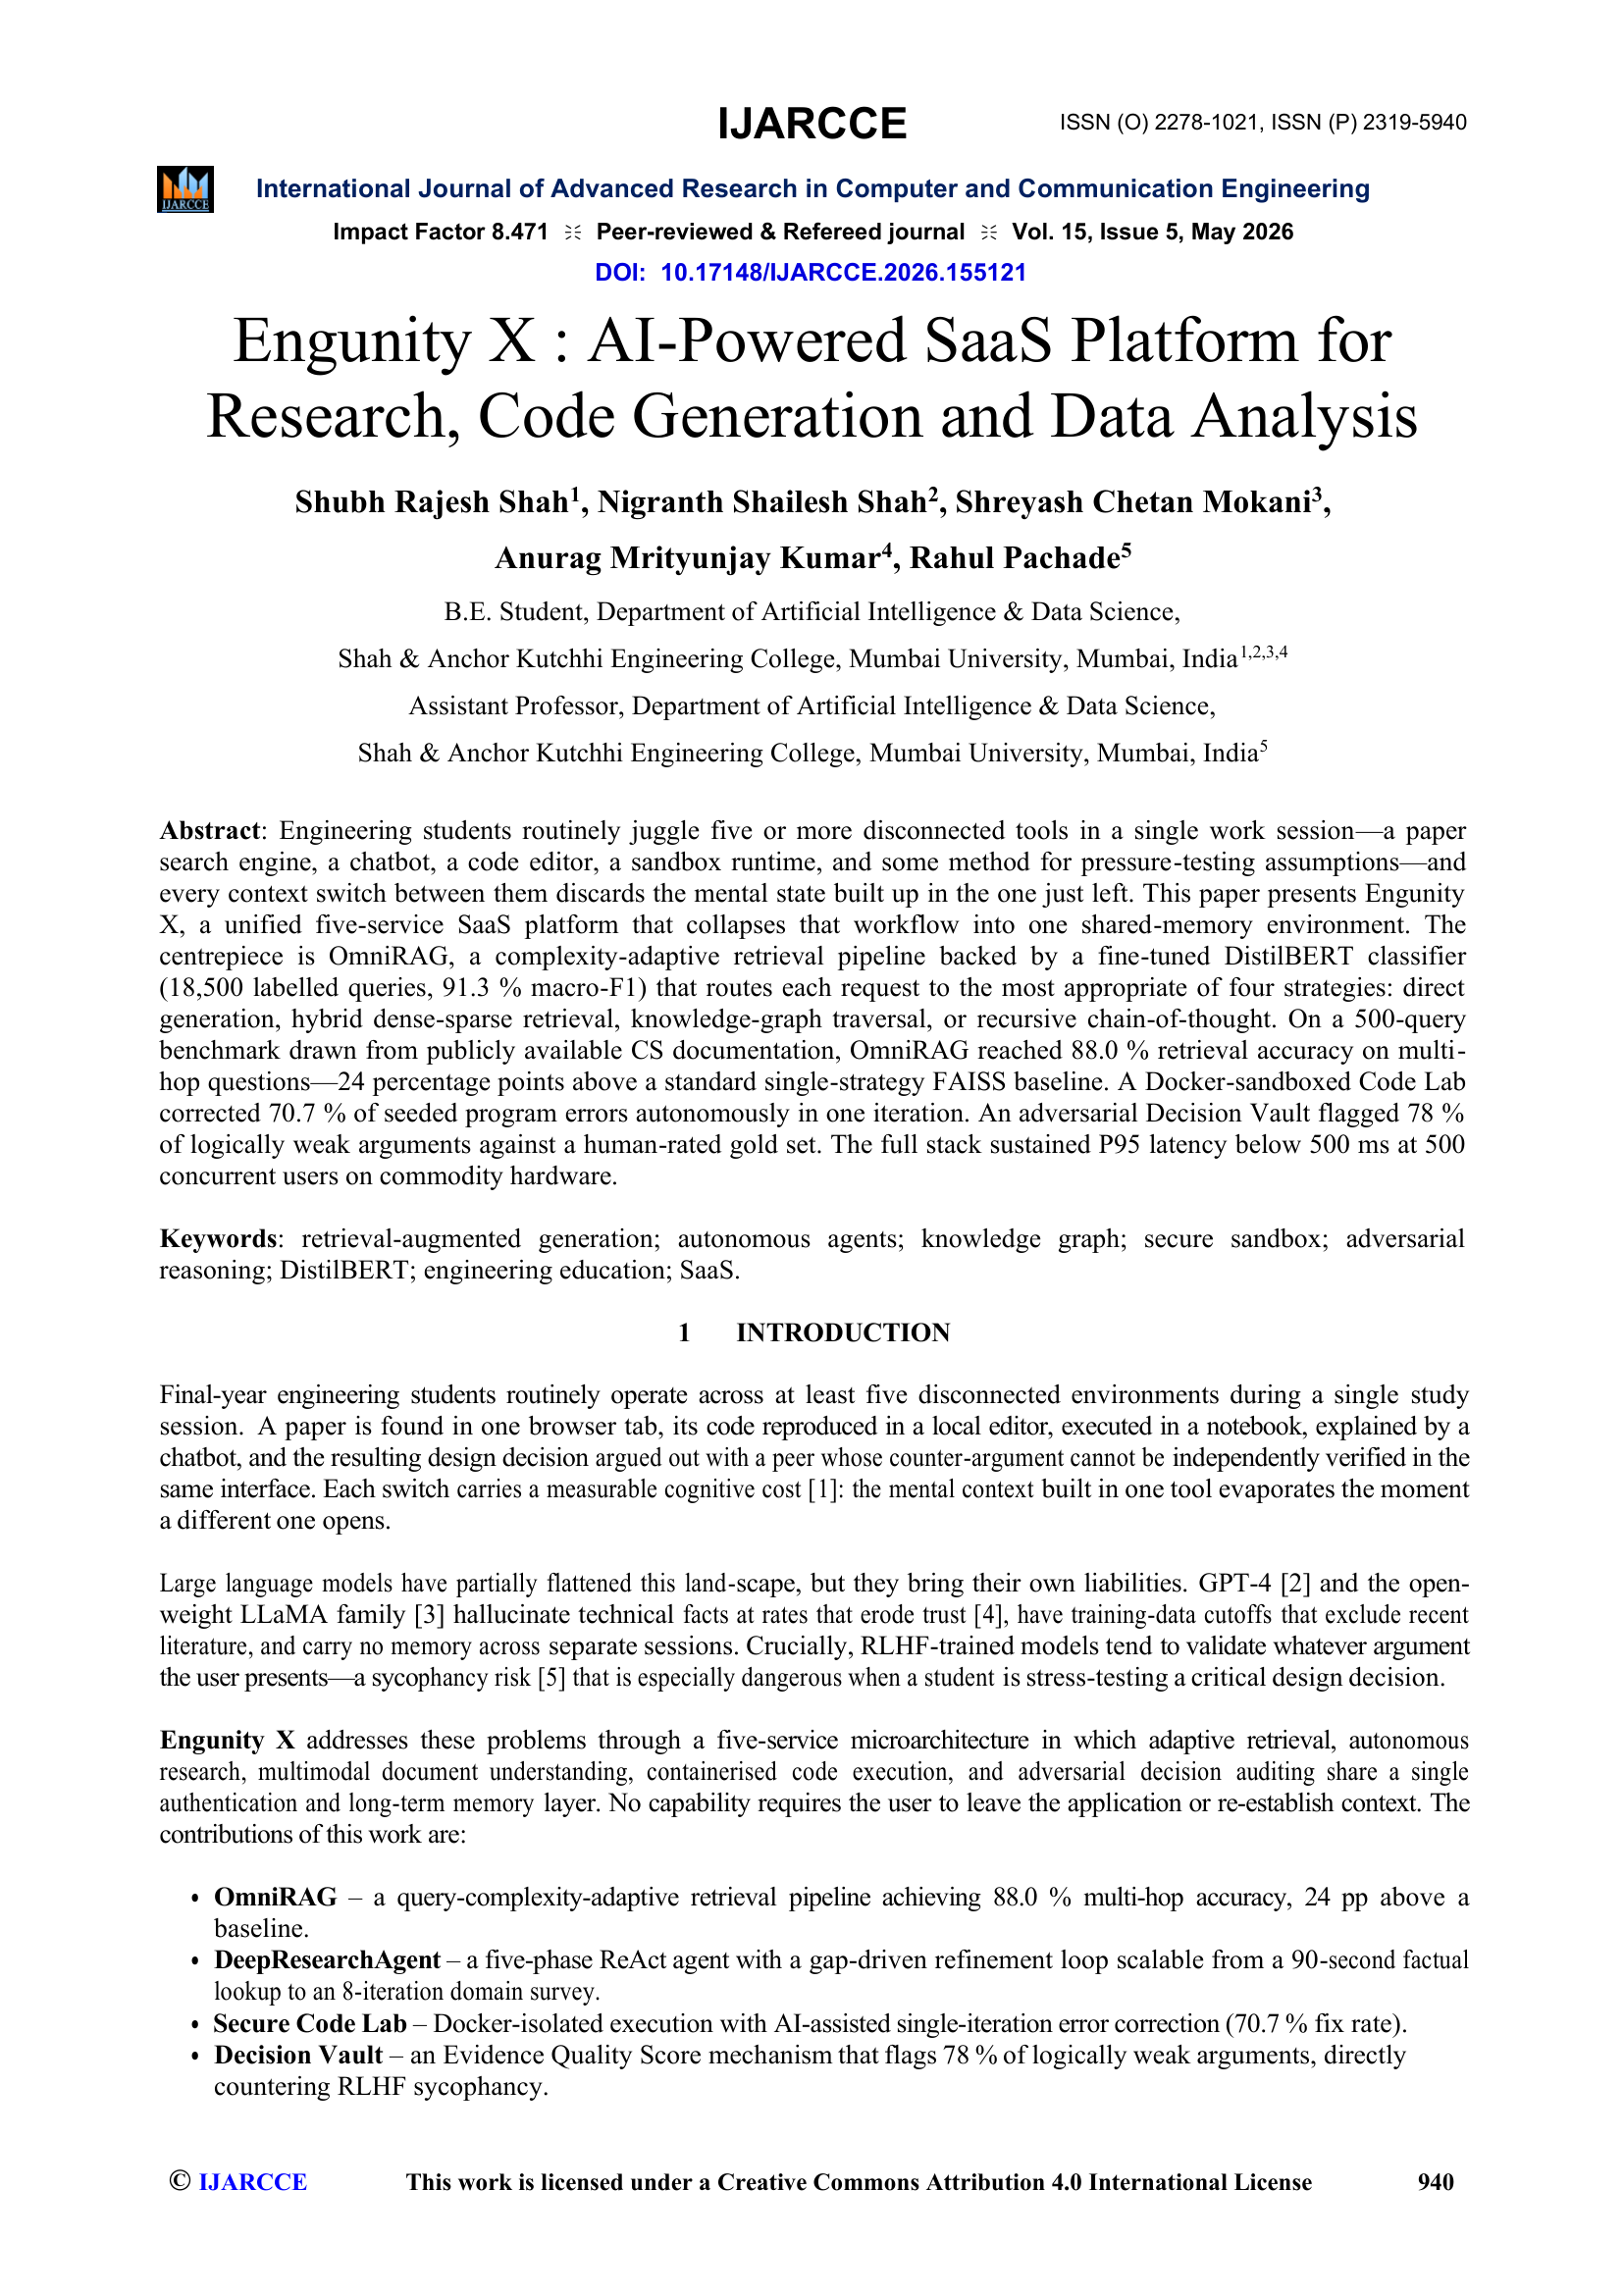
\includegraphics[width=\textwidth,height=\textheight]{./certs_clean/shared_png/research_paper-1.png}%
\par\clearpage

% Page 2
\noindent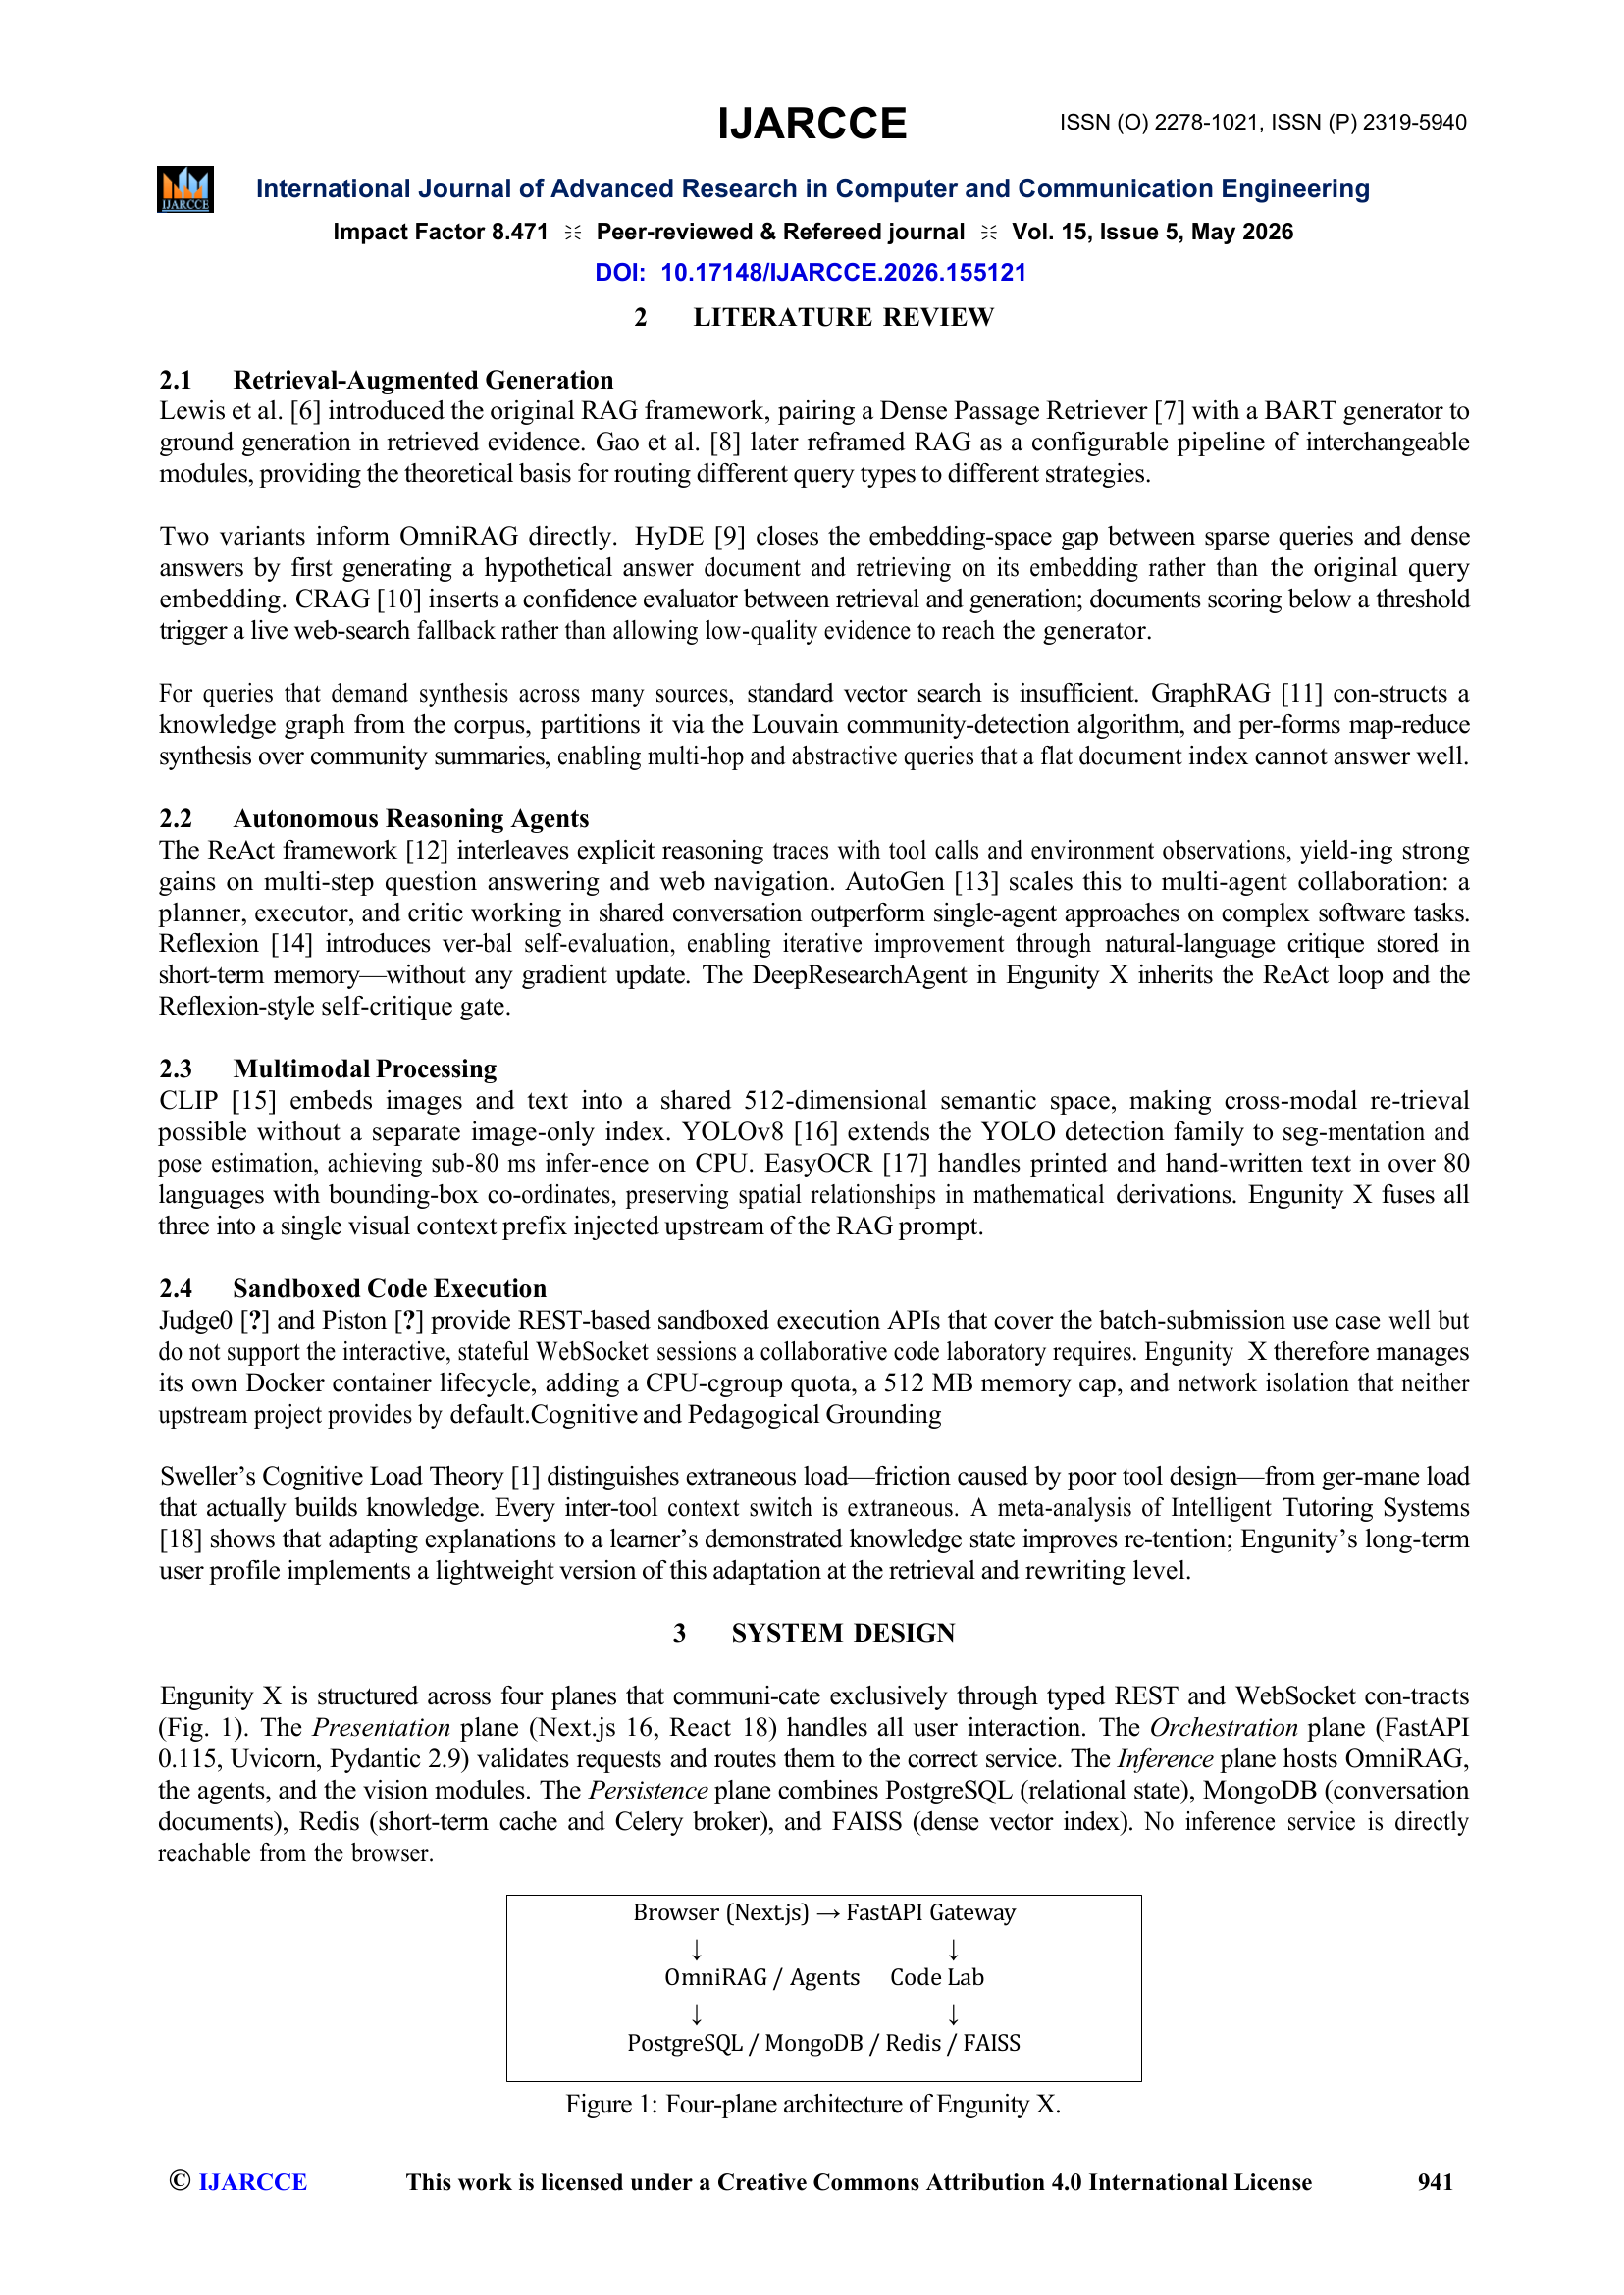
\includegraphics[width=\textwidth,height=\textheight]{./certs_clean/shared_png/research_paper-2.png}%
\par\clearpage

% Page 3
\noindent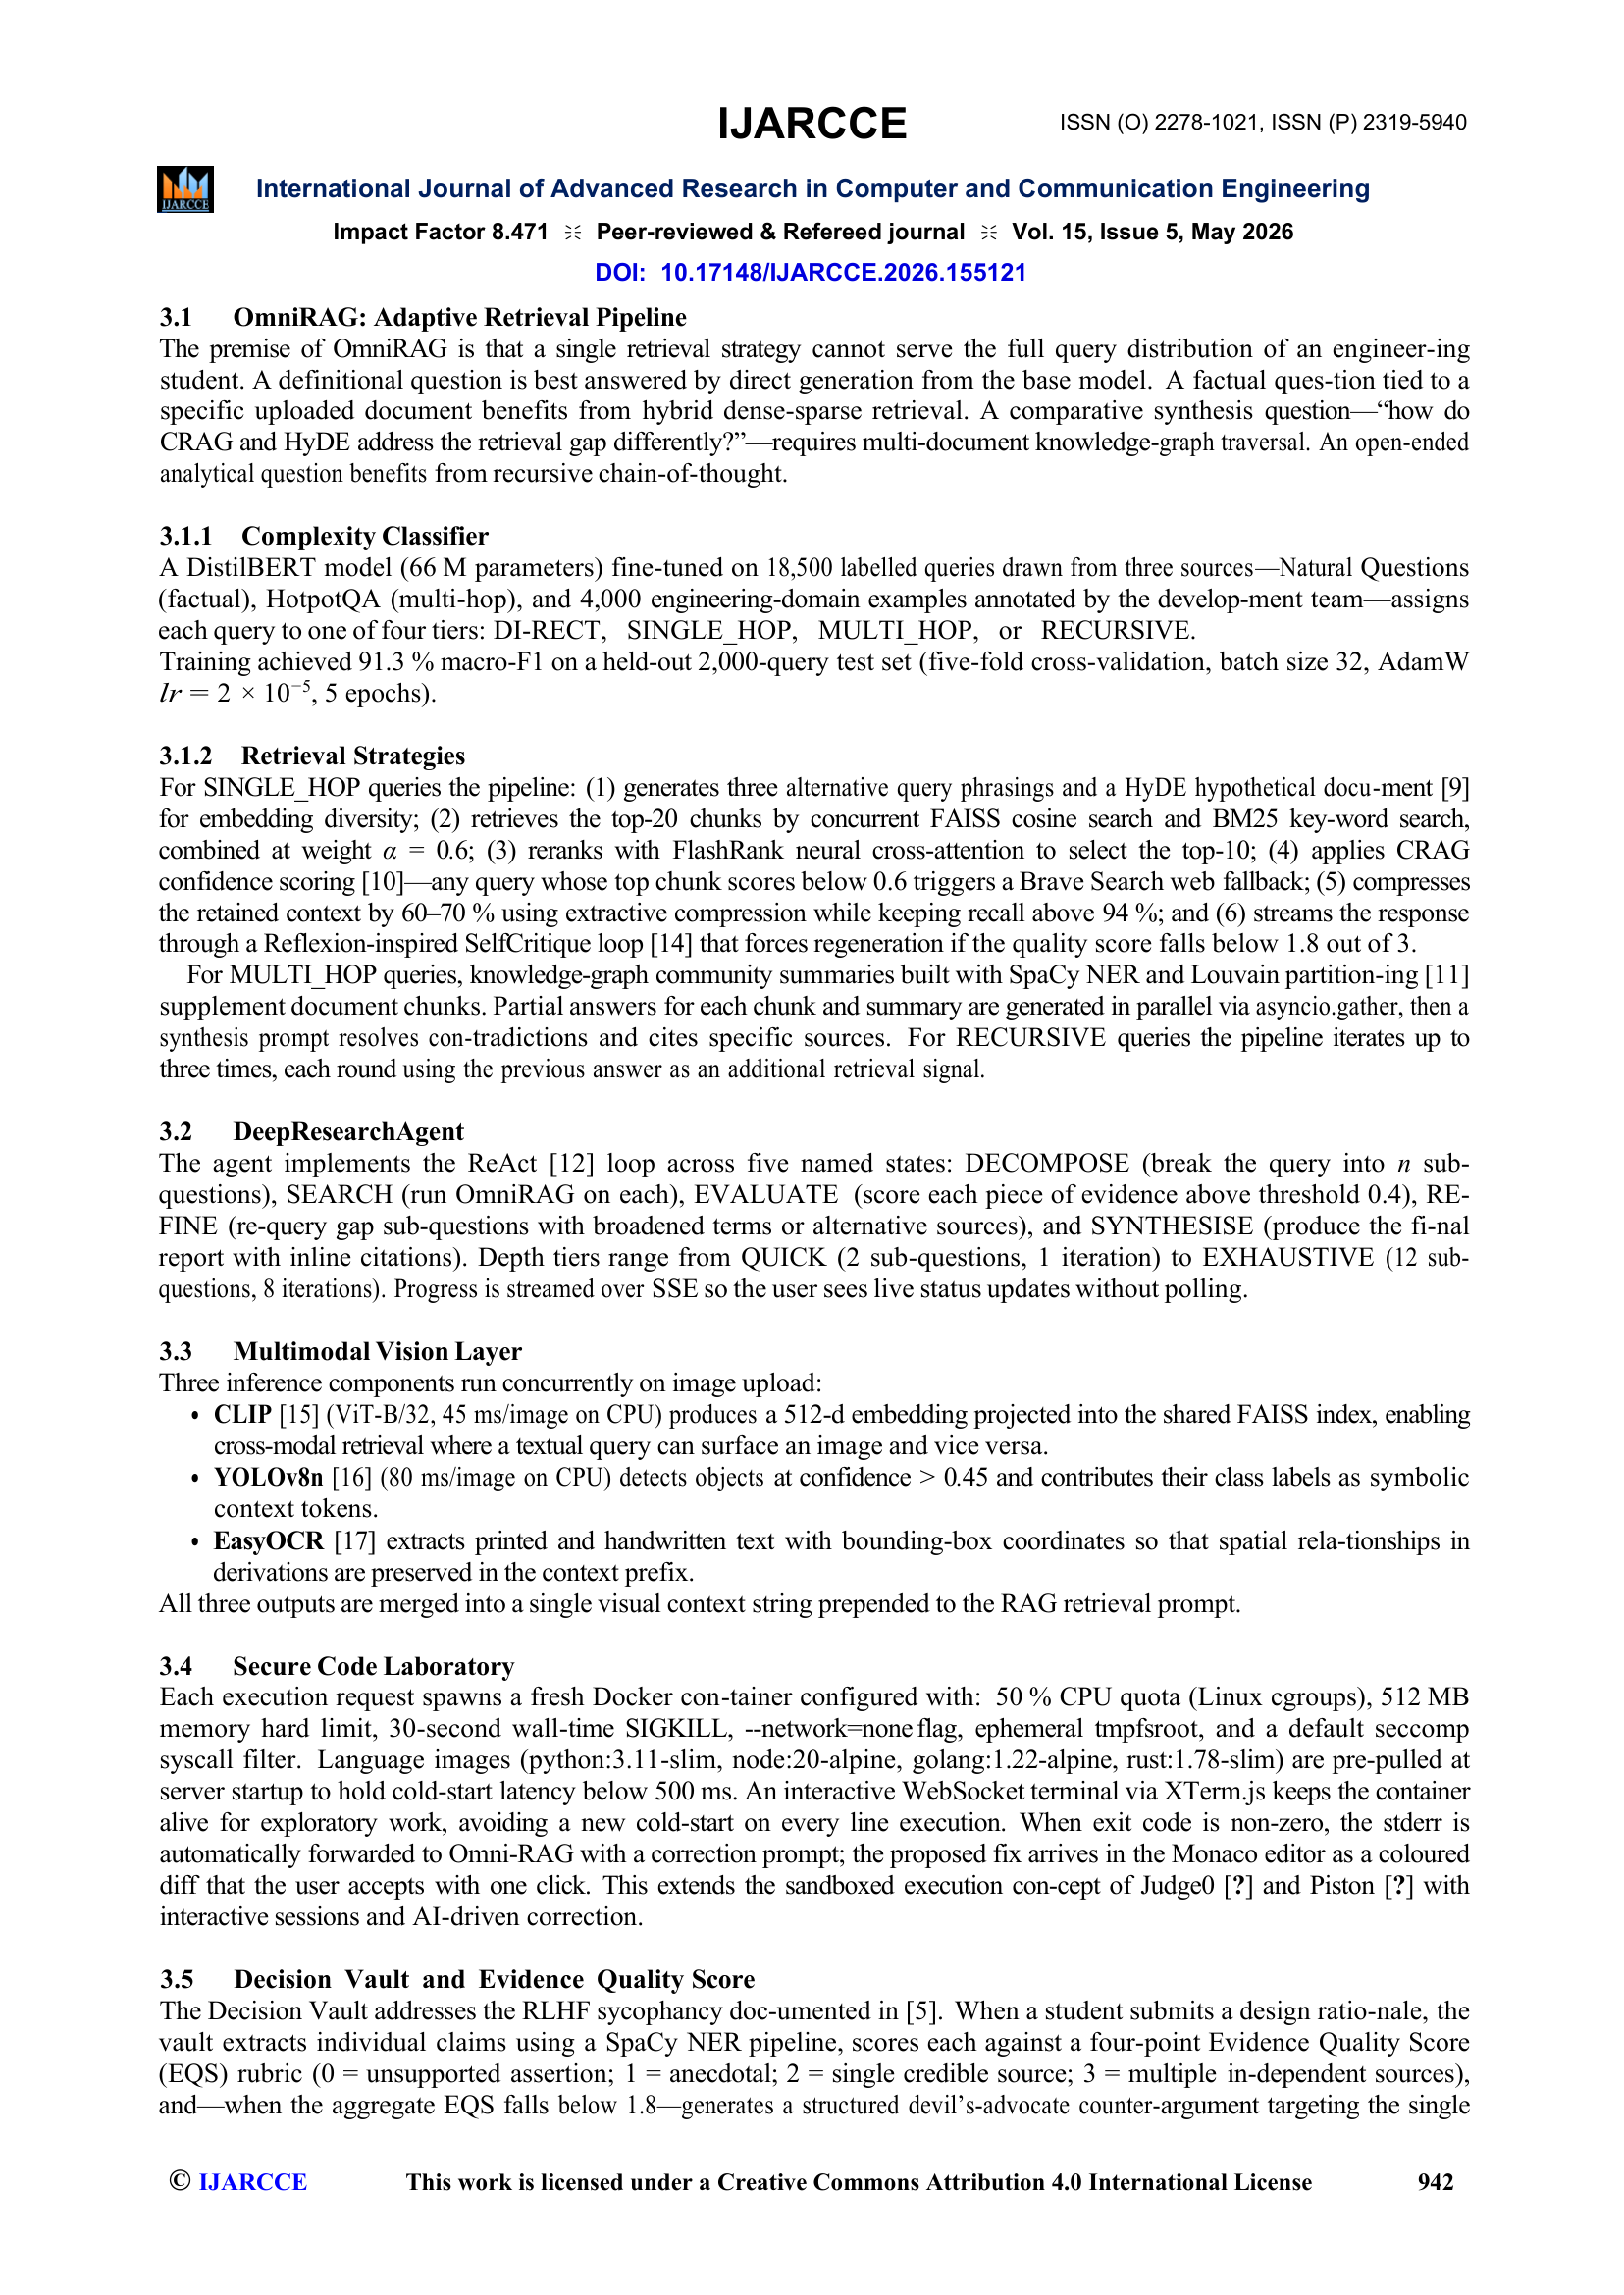
\includegraphics[width=\textwidth,height=\textheight]{./certs_clean/shared_png/research_paper-3.png}%
\par\clearpage

% Page 4
\noindent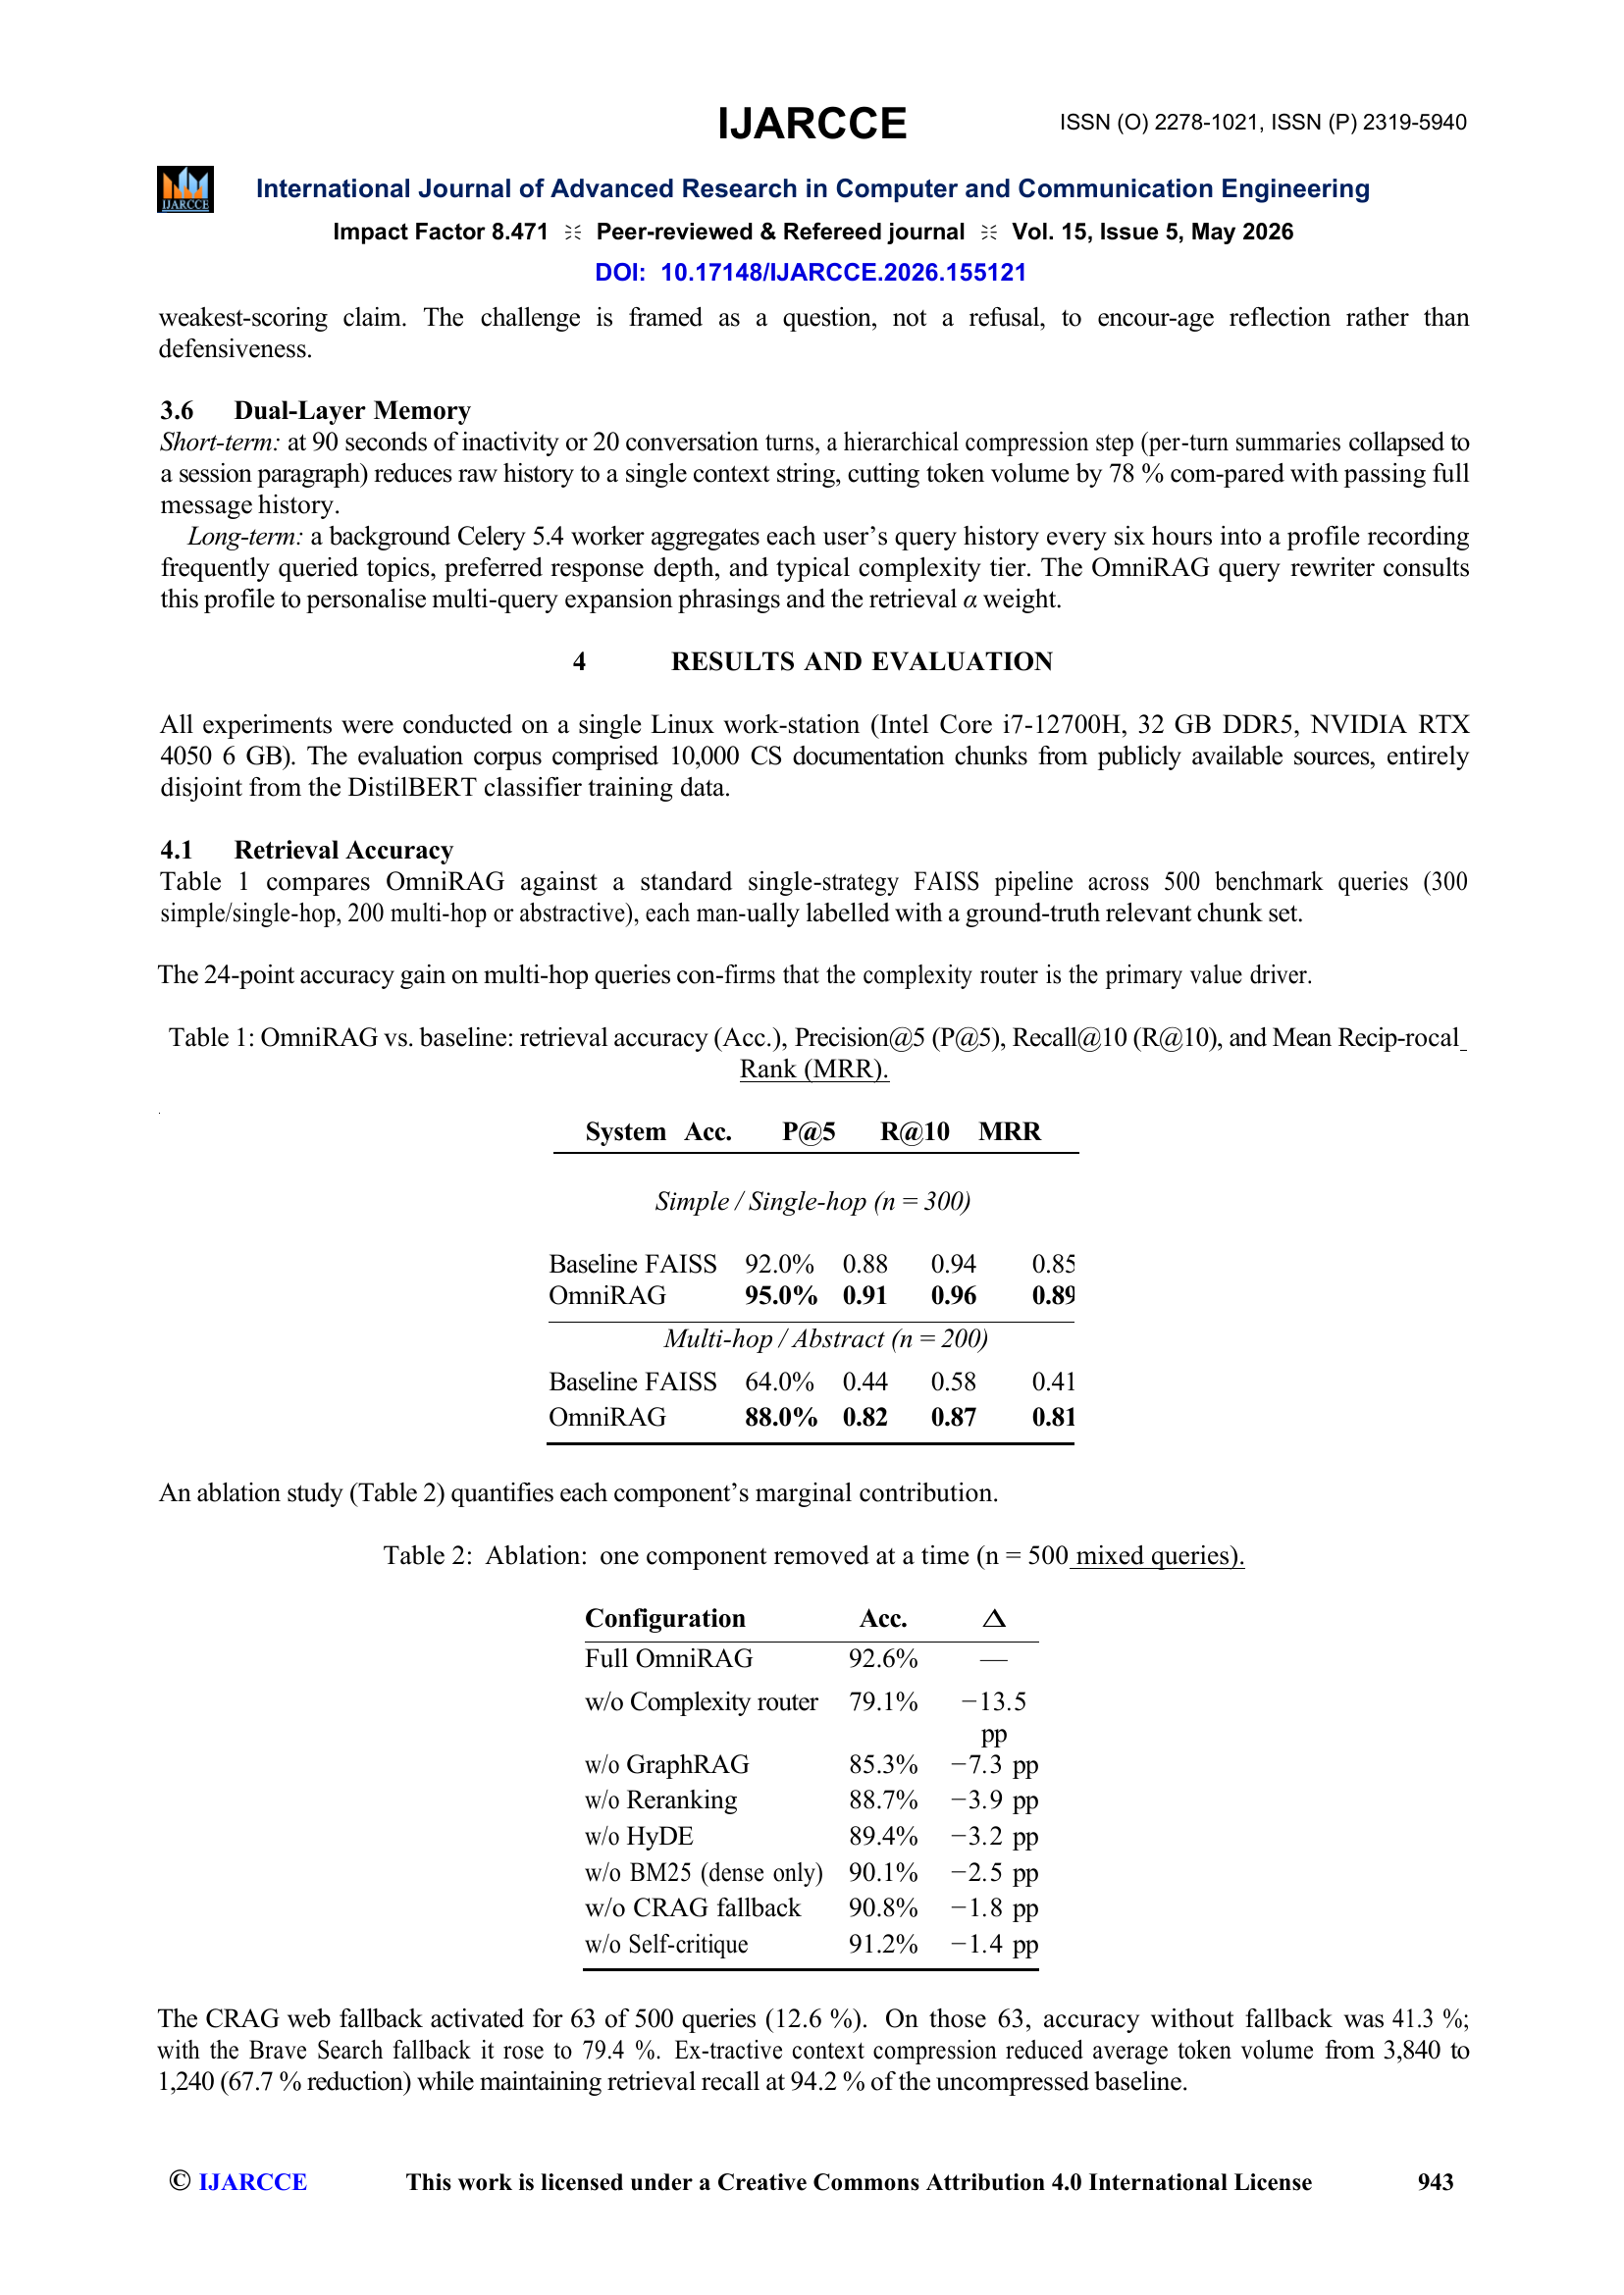
\includegraphics[width=\textwidth,height=\textheight]{./certs_clean/shared_png/research_paper-4.png}%
\par\clearpage

% Page 5
\noindent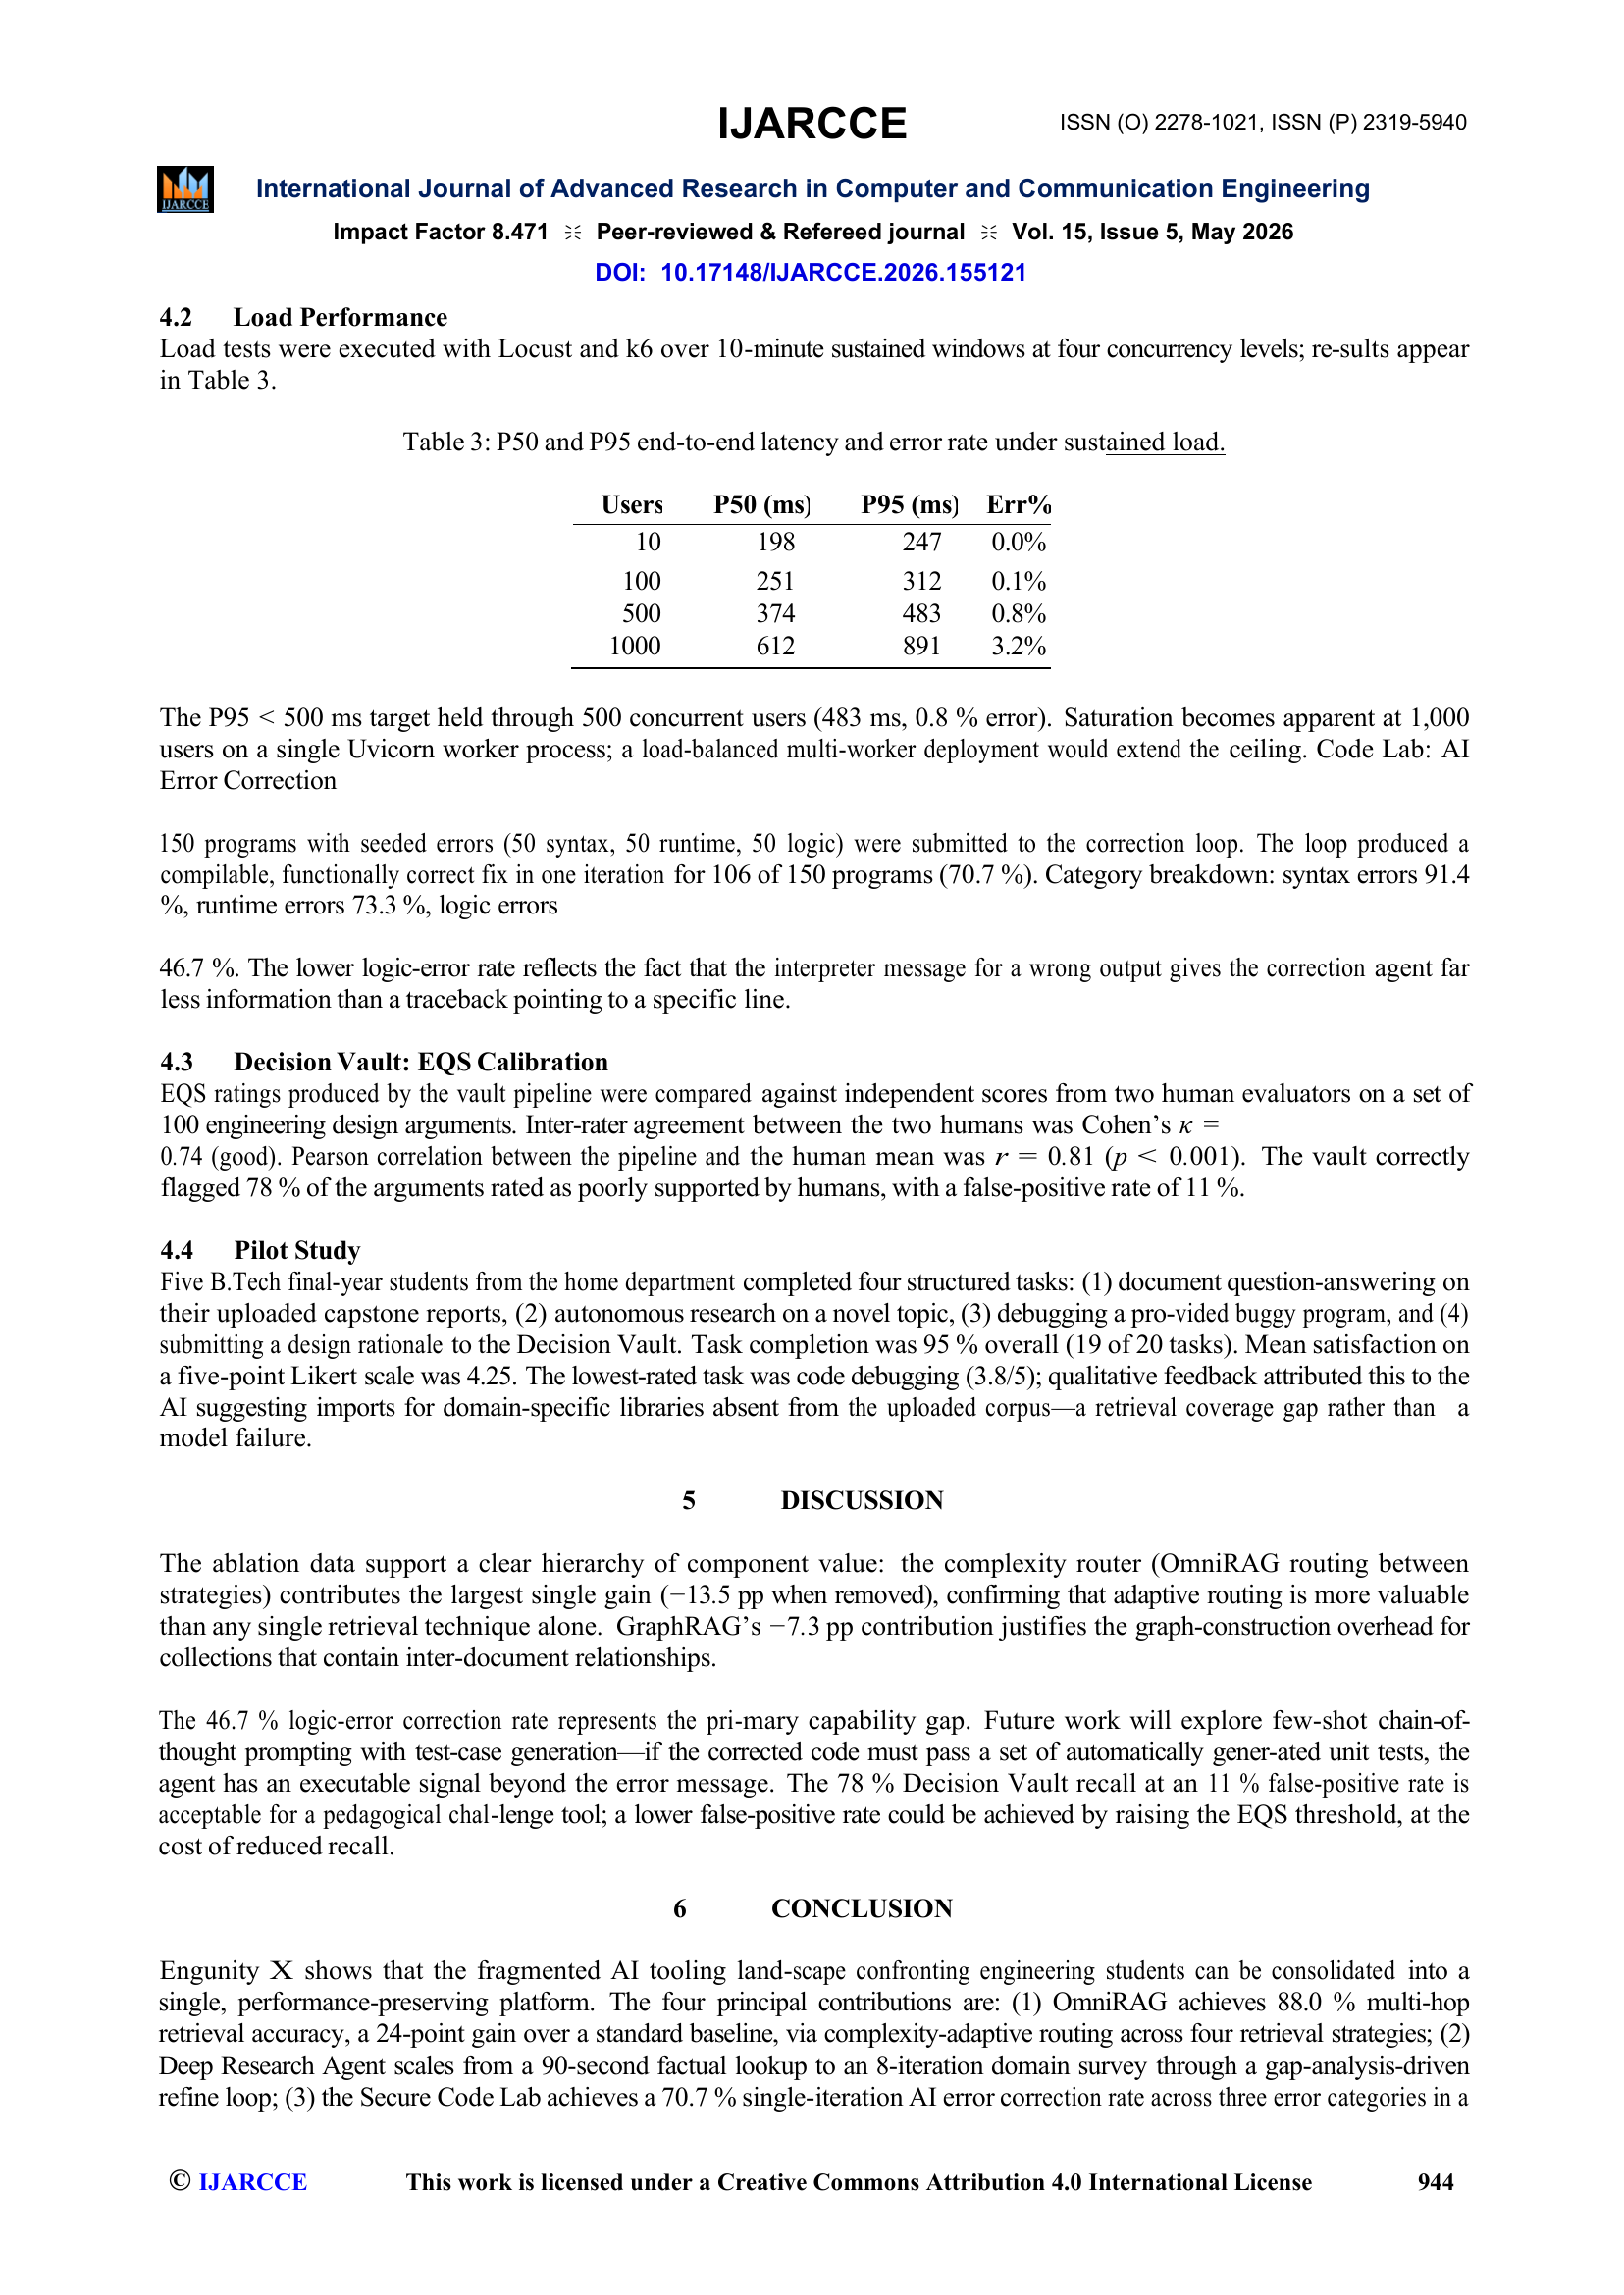
\includegraphics[width=\textwidth,height=\textheight]{./certs_clean/shared_png/research_paper-5.png}%
\par\clearpage

% Page 6
\noindent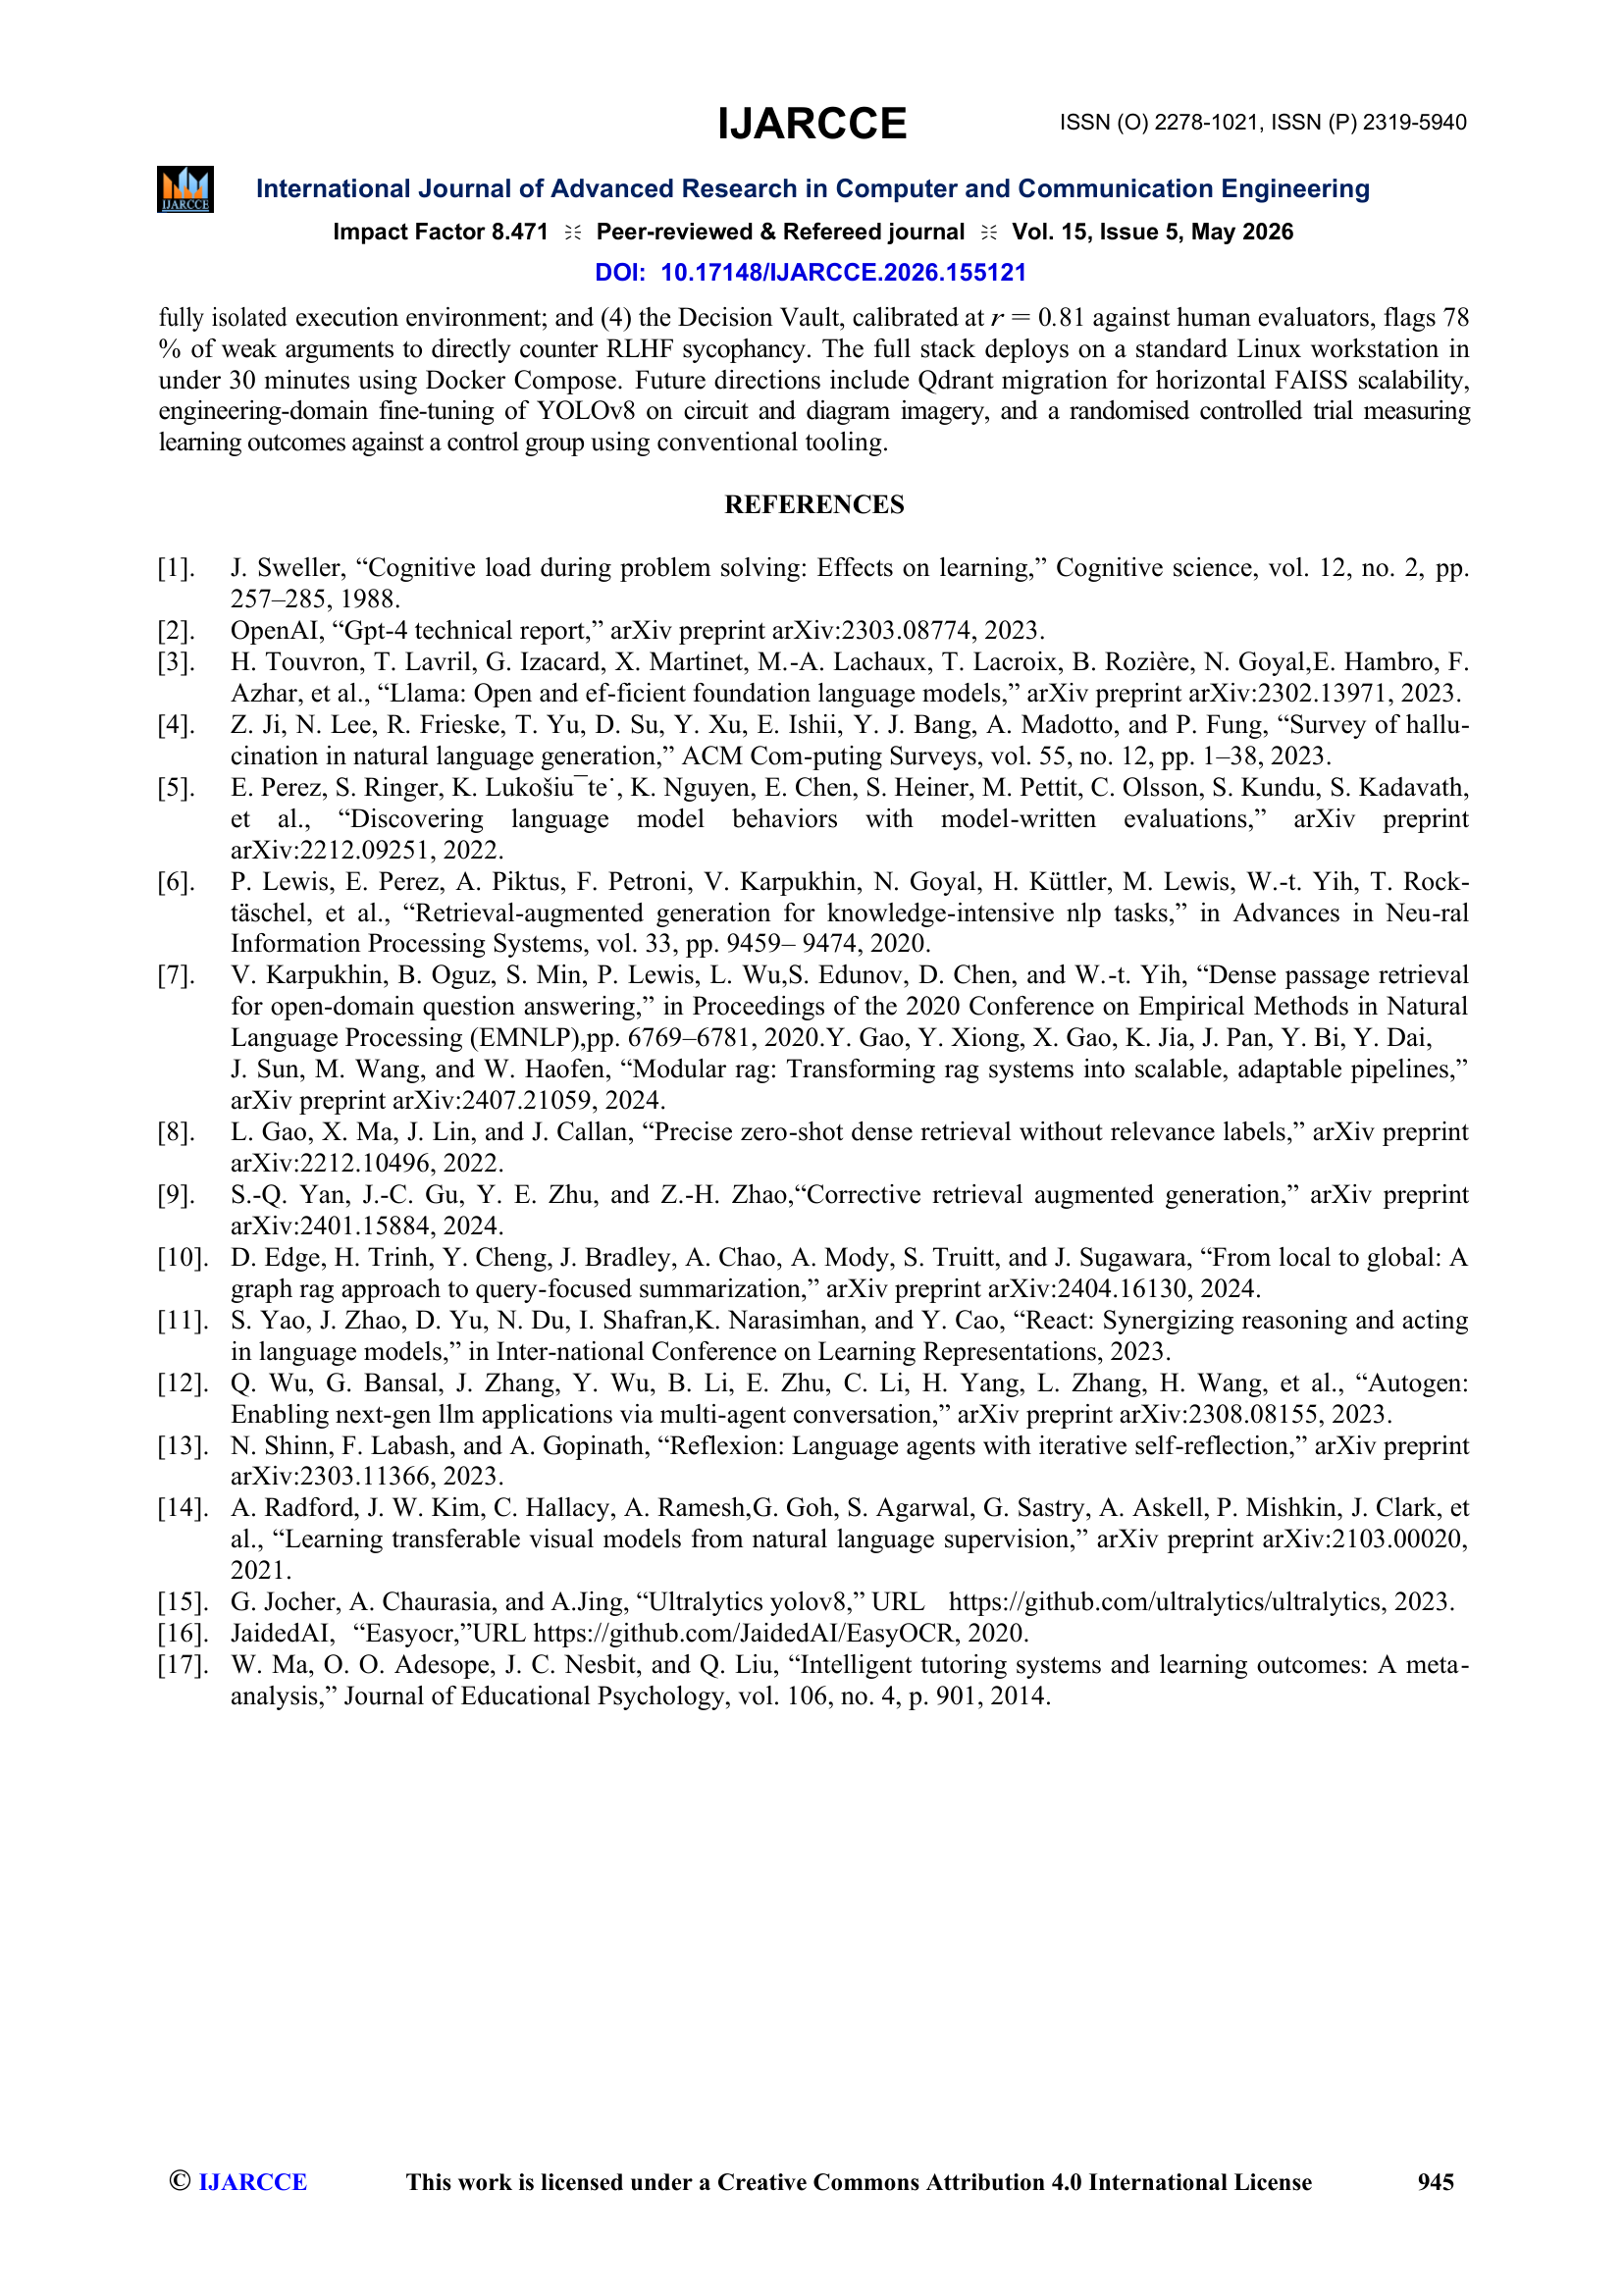
\includegraphics[width=\textwidth,height=\textheight]{./certs_clean/shared_png/research_paper-6.png}%
\par
